\section{Trích xuất Entity và Relationship từ dữ liệu lịch sử}

Phần thực nghiệm này trình bày quy trình trích xuất entity và relationship từ dữ liệu sách giáo khoa lịch sử để xây dựng Knowledge Graph phục vụ hệ thống GraphRAG. Quá trình được thực hiện qua hai giai đoạn chính:
\begin{enumerate}
    \item \textbf{Entity Extraction:} Trích xuất và chuẩn hóa các thực thể lịch sử.
    \item \textbf{Relationship Extraction:} Xác định và trích xuất các mối quan hệ giữa các thực thể.
\end{enumerate}

Cả hai giai đoạn đều sử dụng mô hình ngôn ngữ lớn deepseek-chat kết hợp với kỹ thuật prompt engineering.

%----------------------------------------------------------------------------------------
\subsection{Trích xuất thực thể}
\label{subsec:entity_extraction}
%----------------------------------------------------------------------------------------

Quá trình trích xuất thực thể nhận diện và phân loại các đối tượng có ý nghĩa trong văn bản lịch sử, tuân theo một lược đồ (schema) chuẩn hóa như được định nghĩa trong Bảng \ref{tab:entity_schema}.

\begin{table}[H]
\centering
\caption{Lược đồ (Schema) định nghĩa cho thực thể}
\begin{tabular}{|p{3.2cm}|p{2.5cm}|p{8cm}|}
\hline
\textbf{Trường} & \textbf{Kiểu} & \textbf{Mô tả} \\
\hline
\texttt{id} & String & Định danh duy nhất của thực thể \\
\hline
\texttt{label} & List[String] & Danh sách các tên gọi/biệt danh \\
\hline
\texttt{type} & String & Loại thực thể (11 loại định nghĩa) \\
\hline
\texttt{description} & String & Mô tả ngắn gọn \\
\hline
\texttt{original\_text} & List[Dict] & Vị trí và văn bản gốc mỗi lần xuất hiện \\
\hline
\texttt{properties} & Dict & Thuộc tính có cấu trúc theo chủ đề \\
\hline
\texttt{metadata} & Dict & Thông tin bổ sung (chủ đề, bài học, ...) \\
\hline
\texttt{confidence} & Float & Độ tin cậy (0.0 -- 1.0) \\
\hline
\texttt{occurrence\_count} & Integer & Số lần xuất hiện trong văn bản \\
\hline
\texttt{window\_indices} & List[Int] & Chỉ số cửa sổ văn bản chứa thực thể \\
\hline
\end{tabular}
\label{tab:entity_schema}
\end{table}

\noindent Hệ thống định nghĩa 11 loại thực thể đặc thù cho miền Lịch sử Việt Nam, được liệt kê chi tiết cùng ví dụ trong Bảng \ref{tab:entity_types}.

\begin{table}[H]
\centering
\caption{Các loại thực thể được định nghĩa cho miền lịch sử}
\begin{tabular}{|c|l|p{7.5cm}|}
\hline
\textbf{STT} & \textbf{Loại thực thể} & \textbf{Ví dụ} \\
\hline
1 & Địa điểm & Hà Nội, Điện Biên Phủ, Bến Nhà Rồng \\
\hline
2 & Tổ chức & Liên hợp quốc, ASEAN, Đảng Cộng sản Việt Nam \\
\hline
3 & Khái niệm & Chiến tranh lạnh, Toàn cầu hóa, Đổi mới \\
\hline
4 & Văn kiện/Hiệp định & Hiến chương LHQ, Hiệp định Giơ-ne-vơ \\
\hline
5 & Sự kiện & Cách mạng tháng Tám, Chiến thắng Điện Biên Phủ \\
\hline
6 & Quốc gia & Việt Nam, Liên Xô, Mỹ, Trung Quốc \\
\hline
7 & Chiến lược/Chủ trương & Công nghiệp hóa, Kinh tế thị trường \\
\hline
8 & Hội nghị & Hội nghị I-an-ta, Hội nghị Giơ-ne-vơ \\
\hline
9 & Chiến dịch/Trận đánh & Chiến dịch Điện Biên Phủ, Chiến dịch Hồ Chí Minh \\
\hline
10 & Nhân Vật & Hồ Chí Minh, Võ Nguyên Giáp \\
\hline
11 & Công trình & Lăng Chủ tịch Hồ Chí Minh, Bảo tàng Hồ Chí Minh \\
\hline
\end{tabular}
\label{tab:entity_types}
\end{table}

% Kết quả và Thống kê
\noindent \textbf{Kết quả và Thống kê.} Quá trình trích xuất được thực hiện trên toàn bộ cơ sở tri thức với kết quả tổng hợp về hiệu suất xử lý trong Bảng \ref{tab:extraction_stats} và phân bố chi tiết các loại thực thể trong Bảng \ref{tab:entity_distribution}.

\begin{table}[H]
\centering
\caption{Thống kê hiệu suất quá trình trích xuất thực thể}
\begin{tabular}{|l|r|}
\hline
\textbf{Thông số} & \textbf{Giá trị} \\
\hline
Tổng số chunks (subsections) đầu vào & 76 \\
Tổng số câu văn & 782 \\
Tổng số API requests & 195 \\
Tỷ lệ thành công API & 100\% \\
Thời gian xử lý trung bình/request & 23.51s \\
\hline
Tổng thực thể trước xử lý & 1{,}301 \\
\textbf{Tổng thực thể sau gộp (unique)} & \textbf{625} \\
Tỷ lệ rút gọn (deduplication) & 51.9\% \\
\hline
\end{tabular}
\label{tab:extraction_stats}
\end{table}

\begin{table}[H]
\centering
\caption{Phân bố số lượng thực thể theo loại}
\begin{tabular}{|c|l|r|r|}
\hline
\textbf{STT} & \textbf{Loại thực thể} & \textbf{Số lượng} & \textbf{Tỷ lệ} \\
\hline
1 & Địa điểm & 147 & 23.5\% \\
2 & Tổ chức & 103 & 16.5\% \\
3 & Khái niệm & 86 & 13.8\% \\
4 & Văn kiện/Hiệp định & 59 & 9.4\% \\
5 & Sự kiện & 50 & 8.0\% \\
6 & Quốc gia & 44 & 7.0\% \\
7 & Chiến lược/Chủ trương & 36 & 5.8\% \\
8 & Hội nghị & 30 & 4.8\% \\
9 & Chiến dịch/Trận đánh & 27 & 4.3\% \\
10 & Nhân Vật & 25 & 4.0\% \\
11 & Công trình & 18 & 2.9\% \\
\hline
\multicolumn{2}{|c|}{\textbf{Tổng cộng}} & \textbf{625} & \textbf{100\%} \\
\hline
\end{tabular}
\label{tab:entity_distribution}
\end{table}

% Đánh giá
\noindent \textbf{Đánh giá.}
\begin{itemize}
    \item \textbf{Hiệu suất xử lý:} Tỷ lệ thành công API 100\% và thời gian xử lý trung bình 23.51s cho thấy hệ thống ổn định. Tỷ lệ rút gọn 51.9\% phản ánh hiệu quả của thuật toán gộp thực thể.
    \item \textbf{Chất lượng trích xuất:} Phân bố loại thực thể phù hợp với đặc thù lịch sử. Số lượng Nhân Vật thấp (4.0\%) phản ánh sách giáo khoa ít tập trung tiểu sử cá nhân.
    \item \textbf{Cấu trúc dữ liệu:} Schema được thiết kế hỗ trợ tốt việc truy vết nguồn gốc (\texttt{original\_text}) và khớp nối linh hoạt (\texttt{label} dạng danh sách) tương ứng với các \texttt{context} để có thể dễ dàng truy xuất.
\end{itemize}

%----------------------------------------------------------------------------------------
\subsection{Trích xuất quan hệ}
\label{subsec:relationship_extraction}
%----------------------------------------------------------------------------------------

Quá trình trích xuất quan hệ xác định các mối quan hệ ngữ nghĩa giữa các thực thể đã được trích xuất, chuyển đổi chúng thành một đồ thị tri thức có cấu trúc.

\noindent \textbf{Phương pháp.} Hệ thống sử dụng phương pháp \textbf{Entity-Grounded} và \textbf{Evidence-Based} với các đặc điểm:
\begin{itemize}
    \item Chỉ trích xuất quan hệ giữa các thực thể đã xác định.
    \item Mỗi quan hệ phải có bằng chứng văn bản (evidence) trích xuất trực tiếp.
    \item Sử dụng kỹ thuật \textbf{Semantic Chunking với Overlap} (7 câu/chunk, overlap 5 câu) để không bỏ sót quan hệ ở ranh giới.
    \item Kiểm tra sự tồn tại của subject/object, đảm bảo một relationship được nối với 2 entity khác nhau, loại bỏ quan hệ tự tham chiếu, xác thực độ dài evidence.
\end{itemize}

\noindent \textbf{Định nghĩa quan hệ.} Mỗi quan hệ được biểu diễn dưới dạng bộ ba (triple): \texttt{Subject → Predicate → Object}. Lược đồ (Schema) mô tả chi tiết cho một quan hệ được trình bày trong Bảng \ref{tab:relation_schema}.

\begin{table}[H]
\centering
\caption{Lược đồ (Schema) định nghĩa cho quan hệ}
\label{tab:relation_schema}
\begin{tabular}{|p{3.5cm}|p{2.5cm}|p{7.5cm}|}
\hline
\textbf{Trường} & \textbf{Kiểu} & \textbf{Mô tả} \\
\hline
\texttt{subject\_id} & String & ID thực thể nguồn \\
\hline
\texttt{predicate} & String & Loại quan hệ (ví dụ: \texttt{hop\_tac}) \\
\hline
\texttt{object\_id} & String & ID thực thể đích \\
\hline
\texttt{evidence} & String & Câu văn chứng minh từ nguồn gốc \\
\hline
\texttt{chunk\_info} & Dict & Thông tin vị trí (topic, lesson, section...) \\
\hline
\texttt{occurrence\_count} & Integer & Số lần quan hệ xuất hiện \\
\hline
\texttt{supporting\_sentences} & List[Dict] & Danh sách câu văn hỗ trợ \\
\hline
\texttt{confidence} & Float & Độ tin cậy (0.0 -- 1.0) \\
\hline
\end{tabular}
\end{table}

\noindent \textbf{Kết quả và Thống kê.} Quá trình trích xuất được thực hiện trên 76 chunks gốc (sau chia nhỏ thành 311 chunks) với kết quả tổng hợp về hiệu suất trong Bảng \ref{tab:relation_extraction_stats} và phân bố chi tiết các loại quan hệ (top 10) trong Bảng \ref{tab:relation_distribution}.

\begin{table}[H]
\centering
\caption{Thống kê hiệu suất quá trình trích xuất quan hệ}
\label{tab:relation_extraction_stats}
\begin{tabular}{|l|r|}
\hline
\textbf{Thông số} & \textbf{Giá trị} \\
\hline
Chunks sau chia nhỏ (overlap) & 311 \\
Tổng số API requests & 311 \\
Tỷ lệ thành công API & 100\% \\
\hline
Tổng quan hệ trước validation & $\approx$ 2,800 \\
\textbf{Tổng quan hệ sau validation} & \textbf{1.683} \\
Tỷ lệ quan hệ hợp lệ & $\approx$ 60\% \\
\hline
\end{tabular}
\end{table}

\begin{table}[H]
\centering
\caption{Phân bố quan hệ theo loại predicate (Top 10)}
\label{tab:relation_distribution}
\begin{tabular}{|c|l|r|r|}
\hline
\textbf{STT} & \textbf{Predicate} & \textbf{Số lượng} & \textbf{Tỷ lệ} \\
\hline
1 & \texttt{lien\_quan\_den} & 520 & 29.0\% \\
2 & \texttt{thuoc\_ve} & 124 & 6.9\% \\
3 & \texttt{dien\_ra\_tai} & 119 & 6.6\% \\
4 & \texttt{liên\_quan\_đến} (có dấu) & 116 & 6.5\% \\
5 & \texttt{ket\_qua\_cua} & 94 & 5.2\% \\
6 & \texttt{hop\_tac} & 86 & 4.8\% \\
7 & \texttt{chien\_dau} & 70 & 3.9\% \\
8 & \texttt{tham\_gia} & 69 & 3.8\% \\
9 & \texttt{thong\_qua} & 60 & 3.3\% \\
10 & \texttt{lanh\_dao} & 54 & 3.0\% \\
\hline
\multicolumn{2}{|c|}{\textbf{Các loại khác}} & \textbf{483} & \textbf{26.9\%} \\
\hline
\multicolumn{2}{|c|}{\textbf{Tổng cộng}} & \textbf{1,795} & \textbf{100\%} \\
\hline
\end{tabular}
\end{table}

\noindent \textbf{Đánh giá.}
\begin{itemize}
    \item \textbf{Hiệu quả xử lý:} Pipeline ổn định với 100\% thành công API. Tỷ lệ validation 64\% cho thấy cơ chế lọc hiệu quả. Việc chunking với overlap đảm bảo toàn bộ nội dung đã được duyệt và không bỏ sót câu văn nào.
    \item \textbf{Chất lượng trích xuất:} Quan hệ \texttt{lien\_quan\_den} chiếm tỷ lệ cao nhất (29\%) do tính chất chung đây là relationship được dùng để tạo các mối liên quan giữa các entity trong chủ đề.
    \item \textbf{Hạn chế:} Tồn tại một số mối quan hệ bị trùng nhưng khác cách diễn đạt.
\end{itemize}

\noindent \textbf{Tổng kết Knowledge Graph.} Kết quả cuối cùng của giai đoạn xây dựng đồ thị tri thức (Knowledge Graph) bao gồm:
\begin{itemize}
    \item \textbf{625 thực thể} thuộc 11 loại được định nghĩa.
    \item \textbf{1.608 quan hệ} với nhiềuloại predicates đặc thù miền Lịch sử.
    \item Toàn bộ dữ liệu đồ thị tri thức được xuất ra và lưu trữ dưới định dạng 1 file JSON duy nhất
\begin{figure}
    \centering

\end{figure}\begin{figure}
    \centering
    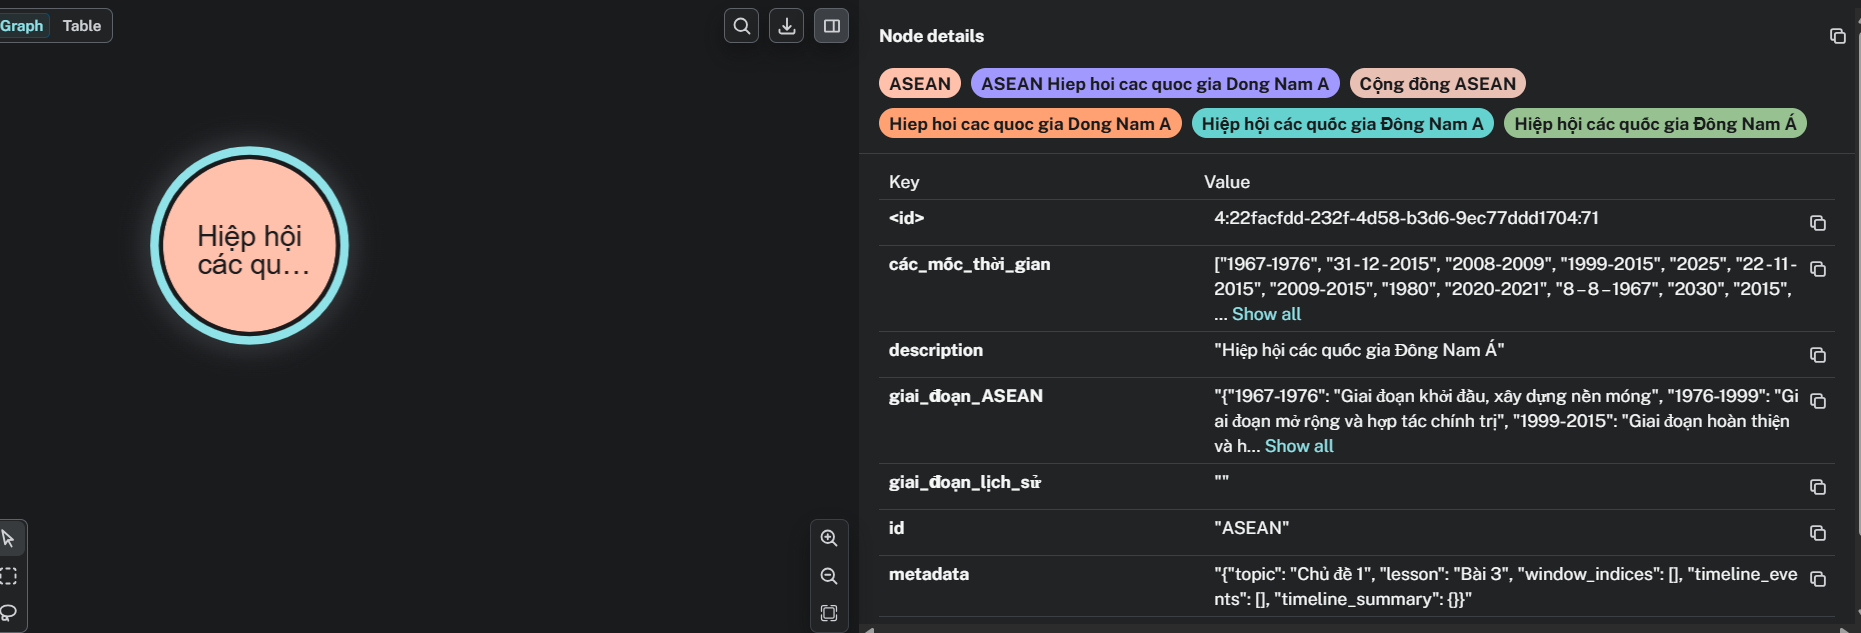
\includegraphics[width=1\linewidth]{image1.png}
    \caption{Ví dụ về entity ASEAN}
    \label{fig:placeholder}
\end{figure}
\begin{figure}
    \centering
    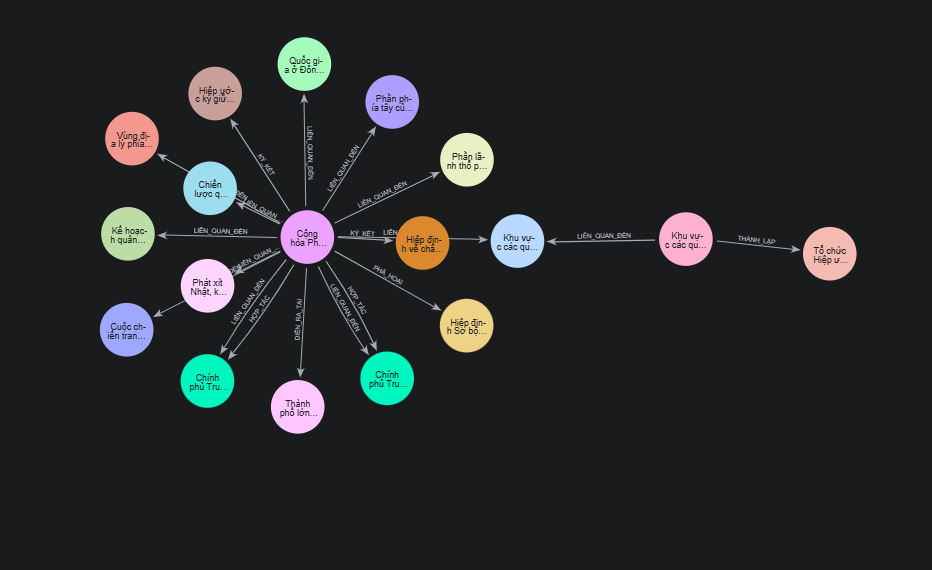
\includegraphics[width=0.6\linewidth]{Screenshot 2025-12-12 222722.png}
    \caption{Ví dụ về entity Pháp và các relationship liền kề}
    \label{fig:placeholder}
\end{figure}
\newpage